\documentclass[border=5pt]{standalone} 
\usepackage{tikz}
\usetikzlibrary{bayesnet}
\usetikzlibrary{arrows}
\usepackage{amsmath}
\begin{document}
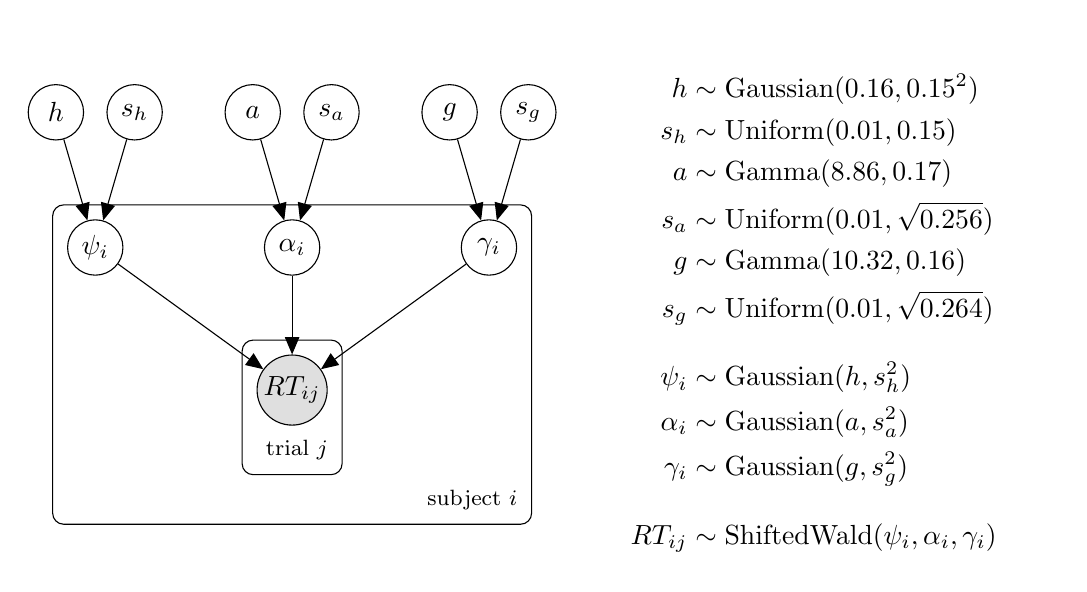
\begin{tikzpicture}

     % nodes
     \node[obs] (y) {$RT_{ij}$};%
     \node[latent, above=of y, xshift=-2.5cm] (psi) {$\psi_{i}$}; %
     \node[latent, above=of y, xshift=0cm] (alpha) {$\alpha_{i}$}; %
     \node[latent, above=of y, xshift=2.5cm] (gamma) {$\gamma_{i}$}; %

     \node[latent, above=of alpha, xshift=-0.5 cm] (a) {$a$}; %
     \node[latent, above=of alpha, xshift=0.5 cm] (sa) {$s_a$}; %

     \node[latent, above=of psi, xshift=-0.5 cm] (h) {$h$}; %
     \node[latent, above=of psi, xshift=0.5 cm] (sh) {$s_h$}; %

     \node[latent, above=of gamma, xshift=-0.5 cm] (g) {$g$}; %
     \node[latent, above=of gamma, xshift=0.5 cm] (sg) {$s_g$}; %
     
     % edges
     \edge {alpha,psi,gamma} {y}
     \edge {a,sa} {alpha}
     \edge {h,sh} {psi}
     \edge {g,sg} {gamma}
     
     % plates

     \plate[inner sep=5pt] {plate1} {(y)} {trial $j$}; %
     \plate[inner sep=5pt] {plate2} {(plate1)(y)(alpha)(psi)(gamma)} {subject $i$}; %

     % text
     \node[text width=6cm, anchor=west, right] at (3.5,1.2)
     {
       \begin{align*}
         h & \sim \text{Gaussian}(0.16, 0.15^2)\\
         s_h & \sim \text{Uniform}(0.01,0.15)\\
     a & \sim \text{Gamma}(8.86, 0.17)\\
         s_a & \sim \text{Uniform}(0.01, \sqrt{0.256})\\
         g & \sim \text{Gamma}(10.32, 0.16)\\
         s_g & \sim \text{Uniform}(0.01, \sqrt{0.264})\\[3mm] 
         \psi_i & \sim \text{Gaussian}(h, s_h^2)\\
        \alpha_i & \sim \text{Gaussian}(a, s_a^2)\\
         \gamma_i & \sim \text{Gaussian}(g, s_g^2)\\[3mm]
         RT_{ij} & \sim \text{ShiftedWald}(\psi_i,\alpha_i, \gamma_i)
       \end{align*}
     };
 \end{tikzpicture}
\end{document}
